% main.tex — ICASSP 2027 submission
% Paper:    Conformal Uncertainty for No-Reference MOS Prediction under Distribution Shift:
%           A Leakage-Controlled Study
% Venue:    ICASSP 2027, Toronto, Canada
% Deadline: September 16, 2026 (HARD)
%
% Compile:  pdflatex main  →  bibtex main  →  pdflatex main  →  pdflatex main
% Style:    spconf.sty (ICASSP/ICIP), IEEEbib.bst (IEEE bibliography)
% -------------------------------------------------------------------------

% Template: ICASSP 2026 (spconf.sty + IEEEbib.bst) — do not change class or style
\pdfminorversion=7
\documentclass{article}
\usepackage{spconf,amsmath,amssymb,graphicx,hyperref,booktabs,microtype,multirow}
\usepackage{balance}

% ---- macros ---------------------------------------------------------------
\newcommand{\qhat}{\hat{q}}
\newcommand{\qtrue}{q^{*}}
\newcommand{\Dtrain}{\mathcal{D}_{\mathrm{train}}}
\newcommand{\Dtest}{\mathcal{D}_{\mathrm{test}}}
\newcommand{\dMx}{d_{M}(\mathbf{x})}
\newcommand{\Calpha}{C_{\alpha}}
\newcommand{\zvec}{\mathbf{z}}
\newcommand{\muvec}{\boldsymbol{\mu}}
\newcommand{\Sigmat}{\boldsymbol{\Sigma}}
\newcommand{\best}[1]{\textbf{#1}}
\newcommand{\second}[1]{\underline{#1}}

% Allow extra inter-word stretch on tight lines (resolves reflow overfull in two-column IEEE layout)
\setlength{\emergencystretch}{1em}

% ---- compact spacing (IEEE two-column) ------------------------------------
\setlength{\textfloatsep}{4pt plus 1pt minus 1pt}
\setlength{\floatsep}{4pt plus 1pt minus 1pt}
\setlength{\intextsep}{3pt plus 1pt minus 1pt}
\setlength{\dbltextfloatsep}{4pt plus 1pt minus 1pt}
\setlength{\dblfloatsep}{4pt plus 1pt minus 1pt}
\setlength{\abovecaptionskip}{0pt}
\setlength{\belowcaptionskip}{0pt}
\setlength{\abovedisplayskip}{4pt plus 1pt minus 1pt}
\setlength{\belowdisplayskip}{4pt plus 1pt minus 1pt}

% Keep bibliography entries at the template's 9-point minimum.
% spconf.sty's \thebibliography prints "\section{References}" then "\list{...}"
% in one call, so \footnotesize must be inserted between them, not before,
% or it also shrinks the section heading (unlike sections 1-5).
\renewcommand{\thebibliography}[1]{%
  \section{References}%
  \small
  \list
    {[\arabic{enumi}]}{\settowidth\labelwidth{[#1]}\leftmargin\labelwidth
     \advance\leftmargin\labelsep
     \usecounter{enumi}}%
  \def\newblock{\hskip .11em plus .33em minus .07em}%
  \sloppy\clubpenalty4000\widowpenalty4000
  \sfcode`\.=1000\relax
  \setlength{\itemsep}{0pt}%
  \setlength{\parskip}{0pt}%
}

% ---- title — ALL CAPS per ICASSP style ----------------------------------
\title{CONFORMAL UNCERTAINTY FOR NO-REFERENCE MOS PREDICTION UNDER DISTRIBUTION SHIFT: A LEAKAGE-CONTROLLED STUDY}

% ---- author block ---------------------------------------------------------
\name{Randy Frans Fela \qquad Pejman Mowlaee}
\address{GN Group, Lautrupbjerg 7, 2750 Ballerup, Denmark}

% ========================================================================
\begin{document}
%\ninept  % 9pt overcorrects (p.5 mostly empty) — reverted, use spacing/trim instead

\maketitle

% --- Abstract (sections/abstract.tex) -----------------------------------
% abstract.tex

\begin{abstract}
No-reference mean opinion score (MOS) predictors output a single number with no signal of trustworthiness, a risk in automated pipelines. We test whether distance from a reference feature distribution can supply that signal, using three frozen predictors, DNSMOS P.835, NISQA, and UTMOS, in a leakage-controlled design that separates feature-reference fitting, content-disjoint calibration, and evaluation across all seven NISQA Corpus subsets. Euclidean, Mahalanobis, and nearest-neighbor distances detect which corpus a clip came from (mean domain AUROC 0.615--0.690) but do not flag which clips carry the largest prediction error within a corpus (mean AUROC 0.433--0.499, near chance). Split conformal intervals built on these distances reach 90.1--91.8\% coverage at the 90\% nominal level with widths of 2.26--2.91 MOS on the four-point scale. Stratifying interval width by Mahalanobis distance helps some predictor--domain pairs and hurts others. This pattern reproduces on an independent multilingual speech-enhancement corpus, so practitioners should read a feature-distance alarm as a domain-mismatch flag, not a per-utterance reliability score.
\end{abstract}


\begin{keywords}
mean opinion score, conformal prediction, out-of-distribution detection,
distribution shift, uncertainty quantification
\end{keywords}

% --- Body sections -------------------------------------------------------
% 01_introduction.tex

\section{Introduction}
\label{sec:intro}

No-reference mean opinion score (MOS) predictors are increasingly used to screen and compare speech systems at scale. DNSMOS P.835~\cite{Reddy2022dnsmos}, NISQA~\cite{Mittag2021nisqa}, and UTMOS~\cite{Saeki2022utmos} reduce reliance on repeated large-scale listening tests, while DNSMOS also serves as an official metric in the DNS Challenge~\cite{dubey2024icassp,Reddy2019scalable}. Their use has outpaced scrutiny of their failure modes.

Existing MOS predictors return point estimates without an explicit reliability measure. A practitioner therefore cannot tell from the score alone whether an utterance should be trusted, reviewed, or sent to a listening test. Feature-space distance is an attractive post-hoc signal because it requires neither predictor retraining nor labelled shifted data. Its interpretation is not automatic, however. A score that recognizes a change in language, channel, or degradation process may still fail to identify which individual MOS predictions are inaccurate.

We test this hypothesis through a conformal uncertainty wrapper for frozen MOS predictors. Split conformal prediction~\cite{Angelopoulos2023conformal} provides finite-sample marginal coverage when calibration and test examples are exchangeable and calibration labels are independent of model fitting. The wrapper first constructs a global interval from calibration residuals. It then applies an established Mondrian-style construction~\cite{Bostrom2020Mondrian} in which Mahalanobis distance~\cite{Lee2018} selects a distance-specific interval radius. The central question is whether a feature-space domain-shift signal transfers to utterance-level error ranking strongly enough to support this adaptation.

This work makes three contributions. First, we construct a leakage-controlled evaluation with disjoint feature-reference, conformal-calibration, and in-domain evaluation roles. Second, we compare Euclidean, Mahalanobis, and nearest-neighbour scores across the distinct tasks of domain detection and utterance-level error detection for three MOS predictors. Third, we test the practical objective directly by comparing fixed and distance-stratified conformal intervals under five metadata-defined shifts. Mean domain-detection AUROC is 0.615--0.690, while mean AUROC for detecting the highest-error quartile is only 0.433--0.499. Distance-stratified interval adaptation is predictor and domain dependent. The contribution is therefore both methodological and empirical, a controlled test showing why an OOD score must be validated as a signal of prediction error, not merely of domain membership, before it is used to adapt prediction uncertainty.

% 02_related_work.tex
\vspace{-.2cm}
\section{Related Work}
\label{sec:related}

Early no-reference speech quality estimators modeled distortion type and signal statistics~\cite{ITUTP563}. NISQA~\cite{Mittag2021nisqa} uses self-attention trained on multi-condition MOS data, DNSMOS P.835~\cite{Reddy2022dnsmos} predicts speech, background, and overall quality by extending the earlier single-score DNSMOS metric~\cite{Reddy2021dnsmos}, and UTMOS~\cite{Saeki2022utmos} builds on self-supervised representations.

OOD detection includes confidence-based~\cite{Hendrycks2017}, density-based, and distance-based methods. Lee et al.~\cite{Lee2018} use class-conditional Mahalanobis distance for image classifiers, and deep nearest-neighbor distance has been evaluated for audio OOD detection~\cite{Bukhsh2023AudioKNN}, following the deep $k$-NN formulation~\cite{Sun2022}. We study a regression analogue based on one Gaussian, compared with Euclidean and nearest-neighbor scores without retraining the predictor, and separately test whether domain discrimination transfers to prediction-error ranking.

Conformal prediction converts residual scores into intervals with finite-sample marginal coverage under exchangeability~\cite{Vovk2005,Angelopoulos2023conformal,Papadopoulos2002}. Mondrian conformal regressors bin a difficulty estimate and calibrate a radius within each bin~\cite{Bostrom2020Mondrian}. Weighted conformal prediction restores a coverage guarantee under a known covariate shift~\cite{Tibshirani2019}, but requires an importance-weight estimate that we do not attempt here. Recent MOS work predicts aleatoric and epistemic uncertainty for selective prediction and domain detection~\cite{Wang2024UncertaintyMOS}, or learns a predictive MOS distribution and filters uncertain samples~\cite{Hoq2025FuseMOS}. We do not present distance binning, audio OOD detection, or MOS selective prediction as new methods. The novelty lies in testing, without retraining or shifted labels, whether internal feature distance transfers across domain detection, utterance-level error ranking, and conformal interval adaptation in frozen speech-quality predictors.

% 03_method.tex
\vspace{-.2cm}
\section{Method}
\label{sec:method}

For a speech waveform $\mathbf{x}$, a frozen no-reference predictor $f$ returns the scalar MOS estimate $\qhat=f(\mathbf{x})$. We extract a fixed-dimensional representation $\zvec=\phi(\mathbf{x})\in\mathbb{R}^{d}$ from each predictor's penultimate layer, mean-pooling frame- or segment-level activations: the second dense layer before the final head for DNSMOS ($d=64$), the self-attention time-dependency module before the pooling heads for NISQA ($d=64$), and the BiLSTM output of the LDConditioner for UTMOS ($d=1024$). Each predictor has its own feature space and therefore its own reference distribution.

\vspace{-.2cm}
\subsection{Feature-Space Scores}
\label{ssec:features}

For each predictor, T-SIM supplies reference features $\{\zvec_i\}_{i=1}^{N}$, where $N=10{,}000$. The maximum-likelihood empirical mean and covariance are
\begin{align}
    \hat{\muvec}
    &= \frac{1}{N}\sum_{i=1}^{N}\zvec_i,
    \label{eq:mean} \\
    \hat{\Sigmat}
    &= \frac{1}{N}\sum_{i=1}^{N}
    (\zvec_i-\hat{\muvec})(\zvec_i-\hat{\muvec})^\top.
    \label{eq:cov}
\end{align}
Here $N>d$ for all predictors, with $d=64$ for DNSMOS and NISQA ($N/d=156$) and $d=1024$ for UTMOS ($N/d=9.8$). We use the empirical covariance throughout and do not apply Ledoit-Wolf shrinkage~\cite{LedoitWolf2004}. At UTMOS's sample size, shrinkage changes AUROC by at most 0.09 (domain) and 0.12 (error), both above the 0.075 spread across scores in Table~\ref{tab:ood-score}, so per-predictor rankings are not resolvable here. The near-chance conclusion of Section~\ref{ssec:detection-results} is unchanged under either estimator. The Mahalanobis score is
\begin{align}
    d_M(\mathbf{x})
    =
    \left[
        (\zvec-\hat{\muvec})^\top
        \hat{\Sigmat}^{-1}
        (\zvec-\hat{\muvec})
    \right]^{1/2}.
    \label{eq:mahal}
\end{align}
We also evaluate Euclidean distance $\lVert\zvec-\hat{\muvec}\rVert_2$ and the distance to the nearest T-SIM representation~\cite{Sun2022}, fixing $k=1$. A repo-only sweep over $k\in\{1,\ldots,50\}$ changes mean AUROC by at most 0.004. A larger score is prespecified to mean farther from the reference distribution. These scores quantify representation shift rather than estimate MOS error.

\vspace{-.2cm}
\subsection{Split Conformal Interval}
\label{ssec:conformal}

V-SIM is partitioned by content identifier into disjoint calibration and in-domain evaluation halves of 1{,}250 clips each. Let
$\mathcal{D}_{\mathrm{cal}}=\{(\mathbf{x}_j,q_j^*)\}_{j=1}^{m}$ denote the calibration half, where $m=1{,}250$ and $q_j^*$ is subjective MOS. The absolute-residual nonconformity score is
\begin{align}
    s_j = \lvert q_j^*-\hat{q}_j\rvert,
    \qquad \hat{q}_j=f(\mathbf{x}_j).
    \label{eq:nonconf}
\end{align}
Let $s_{(1)}\leq\cdots\leq s_{(m)}$ be the ordered calibration scores and let $\alpha\in(0,1)$ denote the miscoverage rate, so nominal coverage is $1-\alpha$ (we use $\alpha=0.10$). For $\alpha\geq 1/(m+1)$, define
\begin{align}
    k_\alpha
    &= \left\lceil(m+1)(1-\alpha)\right\rceil,% \\
    &\hat Q_{1-\alpha} = s_{(k_\alpha)}.
    \label{eq:conformal-quantile}
\end{align}
The fixed-width interval is
\begin{align}
    \Calpha(\mathbf{x})
    =
    [\qhat-\hat Q_{1-\alpha},\,
     \qhat+\hat Q_{1-\alpha}].
    \label{eq:interval}
\end{align}
We do not clip the endpoints to $[1,5]$, since clipping can alter coverage at the scale boundaries. If the calibration examples and a new example are exchangeable and calibration labels were not used to fit or select $f$, then split conformal prediction gives the marginal guarantee
\begin{align}
    \Pr\!\left\{\qtrue\in\Calpha(\mathbf{x})\right\}
    \geq 1-\alpha.
    \label{eq:coverage-guarantee}
\end{align}
The content-disjoint split prevents direct content leakage but does not itself prove exchangeability, which can in principle be tested online~\cite{Vovk2003mondrian}, though we do not conduct that test here. The NISQA model was developed using NISQA Corpus partitions~\cite{Mittag2021nisqa}, so its intervals are treated as empirical rather than as a fresh-data guarantee.

\vspace{-.2cm}
\subsection{Distance-Stratified Interval}
\label{ssec:adaptive}

Following Mondrian conformal regression with binned difficulty estimates~\cite{Bostrom2020Mondrian}, we test whether Mahalanobis distance supports instance-dependent widths. We select Mahalanobis distance because Section~\ref{ssec:detection-results} shows it is comparable to nearest-neighbor distance on domain-detection AUROC while needing only a fixed $(d,d)$ covariance matrix rather than a reference bank that grows with the calibration set. The calibration examples are divided into $K$ empirical quantile bins of $d_M(\mathbf{x})$. Let $I_k$ be the calibration indices assigned to bin $k$, let $m_k=|I_k|$, and let $s_{(r)}^{(k)}$ be the $r$th ordered residual within that bin. For $\alpha\geq1/(m_k+1)$,
\begin{align}
    \ell_{\alpha,k}
    &= \left\lceil(m_k+1)(1-\alpha)\right\rceil, %\\
    &\hat Q_{1-\alpha}^{(k)}=s_{(\ell_{\alpha,k})}^{(k)}.
    \label{eq:bin-quantile}
\end{align} 
If $b(\mathbf{x})\in\{1,\ldots,K\}$ is the bin assigned using the calibration-derived boundaries, then
\begin{align}
    \Calpha^{\mathrm{adapt}}(\mathbf{x})
    =
    [\qhat-\hat Q_{1-\alpha}^{(b(\mathbf{x}))},\,
     \qhat+\hat Q_{1-\alpha}^{(b(\mathbf{x}))}].
    \label{eq:adaptive}
\end{align}
Scores outside the calibration range enter the first or last bin. We use $K=5$ and hold the boundaries and radii fixed at evaluation. Because the boundaries are estimated from the calibration covariates and shifted test examples need not be exchangeable with calibration examples, we treat Eq.~\eqref{eq:adaptive} as a diagnostic post-hoc construction. We do not claim conditional or arbitrary-shift coverage for it.

% 04_experiments.tex

\section{Experiments}
\label{sec:experiments}

\vspace{-.2cm}
\subsection{Setup}
\label{ssec:setup}

We use all seven subsets of the NISQA Corpus~\cite{Mittag2021nisqa}, summarized in Table~\ref{tab:datasets}. T-SIM fits the feature reference statistics and supplies the $k$-NN reference bank. A deterministic content-disjoint split assigns 1{,}250 V-SIM clips to conformal calibration and 1{,}250 to in-domain evaluation. T-LIV, V-LIV, T-FOR, T-TLK, and T-P501 are evaluated as metadata-defined shifts in recording condition, language, or channel. No label from a shifted subset is used for calibration.

\begin{table}[t]
  \centering
  \small
  \renewcommand{\arraystretch}{0.92}
  \caption{NISQA Corpus subsets~\cite{Mittag2021nisqa}. V-SIM splits deterministically into disjoint calibration and in-domain evaluation halves. $N$: clips with MOS labels.}
  \vspace{2pt}
  \label{tab:datasets}
  \resizebox{\columnwidth}{!}{%
  \begin{tabular}{@{}lllr@{}}
    \toprule
    Abbrev. & Subset & Role & $N$ \\
    \midrule
    T-SIM  & \texttt{TRAIN\_SIM}     & Feature reference & 10\,000 \\
    T-LIV  & \texttt{TRAIN\_LIVE}    & Shifted evaluation & 1\,020 \\
    V-SIM-Cal & \texttt{VAL\_SIM}    & Calibration & 1\,250 \\
    V-SIM-ID  & \texttt{VAL\_SIM}    & ID evaluation & 1\,250 \\
    V-LIV  & \texttt{VAL\_LIVE}      & Shifted evaluation & 200 \\
    T-FOR  & \texttt{TEST\_FOR}      & Shifted evaluation & 240 \\
    T-TLK  & \texttt{TEST\_LIVETALK} & Shifted evaluation & 232 \\
    T-P501 & \texttt{TEST\_P501}     & Shifted evaluation & 240 \\
    \bottomrule
  \end{tabular}%
  }
\end{table}


We evaluate DNSMOS P.835~\cite{Reddy2022dnsmos} using its overall-quality output, NISQA v2~\cite{Mittag2021nisqa}, and UTMOS~\cite{Saeki2022utmos}. All outputs are represented on the 1--5 MOS scale. DNSMOS predictions include the non-personalized P.835 polynomial mapping.\footnote{The stored clip-level correction approximates segment-wise mapping for multi-segment clips, with mean absolute discrepancy 0.0038 MOS in a stratified verification sample.} UTMOS scores come from a torchaudio reimplementation of the released checkpoint rather than the pinned fairseq scorer, and we have not verified numerical equivalence between the two.

For point predictions, we report SRCC and RMSE. Domain detection compares each shifted subset with held-out V-SIM using AUROC and FPR at 95\% TPR. V-SIM has no domain-detection bar because it defines the in-domain negative class. Error detection is a separate within-domain task. In each evaluation subset, positives are the highest absolute-error quartile and the score direction is fixed in advance so that larger distance predicts larger error. Figure~\ref{fig:error-auroc} reports group-bootstrap 95\% confidence intervals from 2{,}000 resamples. Interval comparisons independently resample calibration and evaluation groups, then refit quantiles, bin boundaries, and bin-specific radii in every bootstrap replicate.

\vspace{-.2cm}
\subsection{Point Prediction}
\label{ssec:point-results}

Table~\ref{tab:pcc-srcc} shows that a metadata-defined shift does not imply uniform degradation. NISQA was trained on partitions of this corpus, so its numbers are an in-sample reference rather than a generalization test comparable to DNSMOS and UTMOS. UTMOS has the highest SRCC on every subset but reaches RMSE 1.022 on T-TLK. DNSMOS attains nearly the same V-LIV RMSE as NISQA, yet has substantially higher error on T-FOR and T-P501. Rank correlation and scale error therefore provide different views of transfer. Averaging the three point estimates raises SRCC over every single model on both corpora. On URGENT2025, the ensemble mean reaches SRCC 0.674 versus at most 0.597 for any single model.

% tables/tab2_pcc_srcc.tex — Table 2: SRCC + RMSE across shift sequence
% PAPER: Table 2
% NOTE: SRCC higher is better (max 1.0); RMSE lower is better (in MOS units)
% Columns: SIM (in-dist) | T.LIV | V.LIV | FOR | LIVE | P.5 (shifted)
% Values from the canonical score cache. V-SIM uses the held-out 1,250-clip half.
\begin{table}[t]
  \centering
  \small
  \setlength{\tabcolsep}{3.2pt}
  \renewcommand{\arraystretch}{0.92}
  \caption{Point-prediction performance. Higher SRCC and lower RMSE are better. Within each dataset and metric, \best{bold} and \second{underlined} entries are best and second best according to unrounded values. $^\dagger$Entries that round to the same displayed value are ranked by an unrounded difference below 0.001.}
  \vspace{2pt}
  \label{tab:pcc-srcc}
  \resizebox{\columnwidth}{!}{%
  \begin{tabular}{@{}llcccccc@{}}
    \toprule
    & & \multicolumn{1}{c}{Held-out ID} &
    \multicolumn{5}{c}{Shifted evaluation} \\
    \cmidrule(lr){3-3}
    \cmidrule(lr){4-8}
    Model & Metric & V-SIM & T-LIV & V-LIV & T-FOR & T-TLK & T-P501 \\
    \midrule
    \multirow{2}{*}{DNSMOS}
        & SRCC & 0.703 & \second{0.674} & \second{0.674} & 0.541 & 0.593 & 0.695 \\
        & RMSE & \second{0.854} & \second{0.549} & \best{0.525}$^\dagger$ & 0.845 & \second{0.765} & 0.913 \\[2pt]
    \multirow{2}{*}{NISQA}
        & SRCC & \second{0.805} & 0.649 & 0.638 & \second{0.725} & \second{0.706} & \second{0.831} \\
        & RMSE & 0.860 & \best{0.528} & \second{0.525}$^\dagger$ & \second{0.734} & \best{0.747} & \second{0.653} \\[2pt]
    \multirow{2}{*}{UTMOS}
        & SRCC & \best{0.830} & \best{0.702} & \best{0.749} & \best{0.769} & \best{0.773} & \best{0.880} \\
        & RMSE & \best{0.662} & 0.829 & 0.852 & \best{0.604} & 1.022 & \best{0.636} \\
    \bottomrule
  \end{tabular}%
  }
\end{table}


\vspace{-.2cm}
\subsection{Domain Detection Versus Error Detection}
\label{ssec:detection-results}

Table~\ref{tab:ood-score} evaluates domain discrimination. Averaged over 15 predictor--shift pairs, AUROC is 0.615 for Euclidean distance, 0.678 for Mahalanobis distance, and 0.690 for nearest-neighbour distance. Nearest-neighbour distance attains the highest per-predictor AUROC in all three columns, though the margin over Mahalanobis is small for NISQA and negligible for UTMOS, while Mahalanobis obtains the lowest mean FPR@95. Neither score dominates on both metrics, so we treat Mahalanobis and nearest-neighbour distance as comparable alternatives for domain detection.

% tables/tab3_ood_score.tex -- Table 3: OOD score comparison (L2 vs Mahalanobis vs KNN)
% PAPER: Table 3 (ablation)
% AUROC and FPR@95TPR averaged over 5 predeclared shifted subsets:
%   TRAIN_LIVE, VAL_LIVE, TEST_FOR, TEST_LIVETALK, TEST_P501
% ID evaluation set is the held-out VAL_SIM subset (never used to fit reference
% statistics), correcting a self-neighbor leakage issue in k-NN scoring where
% the reference bank previously overlapped the ID evaluation pool.
% Data: eval_auroc_20260814_170658.csv, knn_k_sensitivity_20260814_170806.csv,
%       pca_mahalanobis_ablation_20260814_170828.csv
\begin{table}[t]
  \centering
  \small
  \setlength{\tabcolsep}{3.5pt}
  \renewcommand{\arraystretch}{0.92}
  \caption{Domain detection averaged over five shifted subsets vs. held-out V-SIM (higher AUROC, lower FPR@95 better). \best{Bold}: best per column.}
  \vspace{2pt}
  \label{tab:ood-score}
  \resizebox{\columnwidth}{!}{%
  \begin{tabular}{@{}lccccc@{}}
    \toprule
    & \multicolumn{4}{c}{AUROC $\uparrow$} &
      FPR@95 $\downarrow$ \\
    \cmidrule(lr){2-5}
    OOD score & DNS & NIQ & UTM & Avg. & Avg. \\
    \midrule
    L2 Euclidean
      & 0.585 & 0.693 & 0.569 & 0.615 & 0.854 \\
    Mahalanobis
      & 0.668 & 0.803 & 0.561 & 0.678 & \best{0.732} \\
    $k$-NN ($k=1$)
      & \best{0.697} & \best{0.805} & \best{0.569} & \best{0.690} & 0.763 \\
    \bottomrule
  \end{tabular}%
  }
\end{table}


% Canonical Mahalanobis K=5 intervals calibrated on one V-SIM half.
% PAPER: Table 4
\begin{table}[t]
  \centering
  %\small
  \footnotesize
  \setlength{\tabcolsep}{0.8pt}
  \renewcommand{\arraystretch}{0.94}
  \caption{Coverage (Cov., \%) and mean width (W) at 90\% nominal coverage. Fixed (F) and five-bin Mahalanobis-adaptive (A) intervals use the same V-SIM calibration split. Interpret coverage and width jointly. %Neither alone determines the better interval.
  }
  \vspace{2pt}
  \label{tab:coverage}
  \begin{tabular}{@{}l*{6}{cc}@{}}
    \toprule
    & \multicolumn{4}{c}{DNSMOS} & \multicolumn{4}{c}{NISQA} &
    \multicolumn{4}{c}{UTMOS} \\
    \cmidrule(lr){2-5}\cmidrule(lr){6-9}\cmidrule(lr){10-13}
    Dataset
    & \multicolumn{2}{c}{F} & \multicolumn{2}{c}{A}
    & \multicolumn{2}{c}{F} & \multicolumn{2}{c}{A}
    & \multicolumn{2}{c}{F} & \multicolumn{2}{c}{A} \\
    \cmidrule(lr){2-3}\cmidrule(lr){4-5}
    \cmidrule(lr){6-7}\cmidrule(lr){8-9}
    \cmidrule(lr){10-11}\cmidrule(lr){12-13}
    & Cov. & W & Cov. & W
    & Cov. & W & Cov. & W
    & Cov. & W & Cov. & W \\
    \midrule
    V-SIM
      & 90.2 & 2.74 & 90.1 & 2.73
      & 90.1 & 2.91 & 89.4 & 2.83
      & 91.8 & 2.26 & 92.1 & 2.28 \\
    T-LIV
      & 99.0 & 2.74 & 98.6 & 2.63
      & 99.3 & 2.91 & 94.3 & 2.16
      & 81.3 & 2.26 & 82.1 & 2.31 \\
    V-LIV
      & 100.0 & 2.74 & 99.5 & 2.63
      & 99.5 & 2.91 & 98.0 & 2.14
      & 78.0 & 2.26 & 79.0 & 2.31 \\
    T-FOR
      & 90.0 & 2.74 & 87.9 & 2.67
      & 92.9 & 2.91 & 90.8 & 2.54
      & 92.1 & 2.26 & 93.3 & 2.32 \\
    T-TLK
      & 94.4 & 2.74 & 93.5 & 2.63
      & 93.5 & 2.91 & 84.1 & 2.21
      & 66.4 & 2.26 & 67.7 & 2.31 \\
    T-P501
      & 85.8 & 2.74 & 87.1 & 2.72
      & 97.1 & 2.91 & 90.4 & 2.50
      & 92.1 & 2.26 & 91.2 & 2.32 \\
    \bottomrule
  \end{tabular}
\end{table}

\begin{figure}[t]
  \centering
  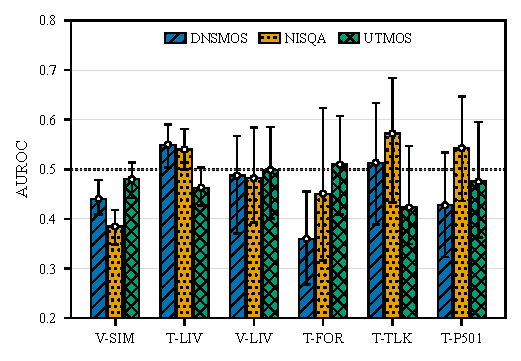
\includegraphics[width=\columnwidth]{figures/auroc_bar.pdf}
  \vspace{-.8cm}
  \caption{Within-domain detection of the highest absolute-error quartile using Mahalanobis distance. Color and hatch encode the predictor. Points show AUROC estimates and error bars show group-bootstrap 95\% confidence intervals from 2{,}000 resamples. V-SIM is included because this is error detection rather than domain discrimination. %The dotted line denotes chance performance.
  }
  \label{fig:error-auroc}
\end{figure}

Figure~\ref{fig:error-auroc} shows that domain discrimination and error detection are not interchangeable. Across the 18 predictor--subset pairs, mean error-detection AUROC is 0.478 for Mahalanobis distance. The corresponding means are 0.433 for Euclidean distance, 0.499 for nearest-neighbour distance, and 0.421 for prediction extremity $|\qhat-3|$. On T-LIV, Mahalanobis AUROC is 0.549 for DNSMOS, 0.540 for NISQA, and 0.463 for UTMOS. DNSMOS on T-FOR reaches only 0.360 with 95\% CI $[0.268,0.455]$, and NISQA on its own held-out V-SIM half reaches 0.385 with CI $[0.349,0.418]$, an equally sub-chance and even tighter interval on the model's in-sample data. Spearman correlation between $\dMx$ and $|\qhat-\qtrue|$ within each subset, a continuous rank-correlation check, agrees qualitatively with the AUROC-based conclusion: correlations are small and inconsistent in sign across predictors and subsets. A single higher-distance-means-higher-error rejection rule is therefore not transferable.

Applying the NISQA-Corpus-fitted Mahalanobis, Euclidean, and nearest-neighbour references, without refitting, to 364 clips from the Interspeech 2025 URGENT Challenge~\cite{Sach2025} (six languages, 26 enhancement systems) gives domain-detection AUROC up to 0.911 against held-out V-SIM but error-detection AUROC of only 0.415 to 0.541. This dissociation is not specific to NISQA Corpus.

\vspace{-.2cm}
\subsection{Conformal Intervals}
\label{ssec:interval-results}

Table~\ref{tab:coverage} reports the fixed and five-bin Mahalanobis-adaptive intervals. Fixed coverage on held-out V-SIM is 90.2\%, 90.1\%, and 91.8\% for DNSMOS, NISQA, and UTMOS. This confirms the expected in-domain behavior of the disjoint calibration design. Fixed widths span 2.26 to 2.91 MOS, 56--73\% of the four-point (1--5) scale, so the coverage guarantee is bought with intervals that occupy most of the usable range. Coverage under shift ranges from 66.4\% to 100.0\%, which is consistent with the absence of an arbitrary-shift guarantee.

Adaptation is predictor and domain dependent. For NISQA, coverage changes from 97.1\% to 90.4\% on T-P501 and from 93.5\% to 84.1\% on T-TLK. Both changes have bootstrap CIs that exclude zero. $k$-NN and Euclidean bins avoid this T-TLK undercoverage. The evidence does not support a better wrapper.
% 05_conclusion.tex

\section{Conclusion}
\label{sec:conclusion}

Feature-space distance separates some corpus shifts, but its association with prediction error is weak and can reverse direction. Mahalanobis-stratified intervals therefore improve some predictor--domain pairs and harm others. This dissociation also appears on an independent corpus.

Feature-distance alarms indicate corpus mismatch, not unreliable predictions without predictor- and domain-specific validation. Fixed split conformal intervals provide matched-domain marginal coverage under exchangeability and independent calibration. Arbitrary shift has no coverage guarantee.

Scorer fidelity is a limitation: our UTMOS reimplementation and DNSMOS segment-length approximation have unverified equivalence to their reference implementations, and results may differ for other predictors, distances, or domains. Future work should test learned, error-supervised difficulty scores and calibration conditioned on validated domain labels, rather than unsupervised feature distance alone.


% --- References ----------------------------------------------------------
\balance
\bibliographystyle{IEEEbib}
\bibliography{strings,refs}

\end{document}
